\documentclass[10pt]{beamer}

\usepackage{appendixnumberbeamer}
\usepackage{booktabs}
\usepackage[scale=2]{ccicons}
\usepackage{pgfplots}
\usepackage{graphics}
\usepackage{braket}

\usepgfplotslibrary{dateplot}
\pdfstringdefDisableCommands{\def\translate#1{#1}}
\geometry{paperwidth=140mm, paperheight=105mm}
\usetheme{metropolis}
\bibliographystyle{abbrv}
\setbeamertemplate{frame footer}{ME738 - Special Topics in Materials}

\renewcommand{\footnotesize}{\fontsize{7pt}{8pt}\selectfont}

\title{Chip Scale Atomic Clocks Sources}
\subtitle{Future developments}
\date{March 5, 2024}
\author{Tommaso Bocchietti}
\institute{University of Waterloo}
\titlegraphic{\hfill
\includegraphics[height=1.5cm]{pdf/UniversityOfWaterloo_logo_horiz_pms.pdf}}

\begin{document}

\maketitle


\appendix

% \begin{frame}[standout]
    Extra slides
\end{frame}



\begin{frame}{$\mathrm{NO_x}$ Emissions}

    \begin{figure}[H]
        \centering
        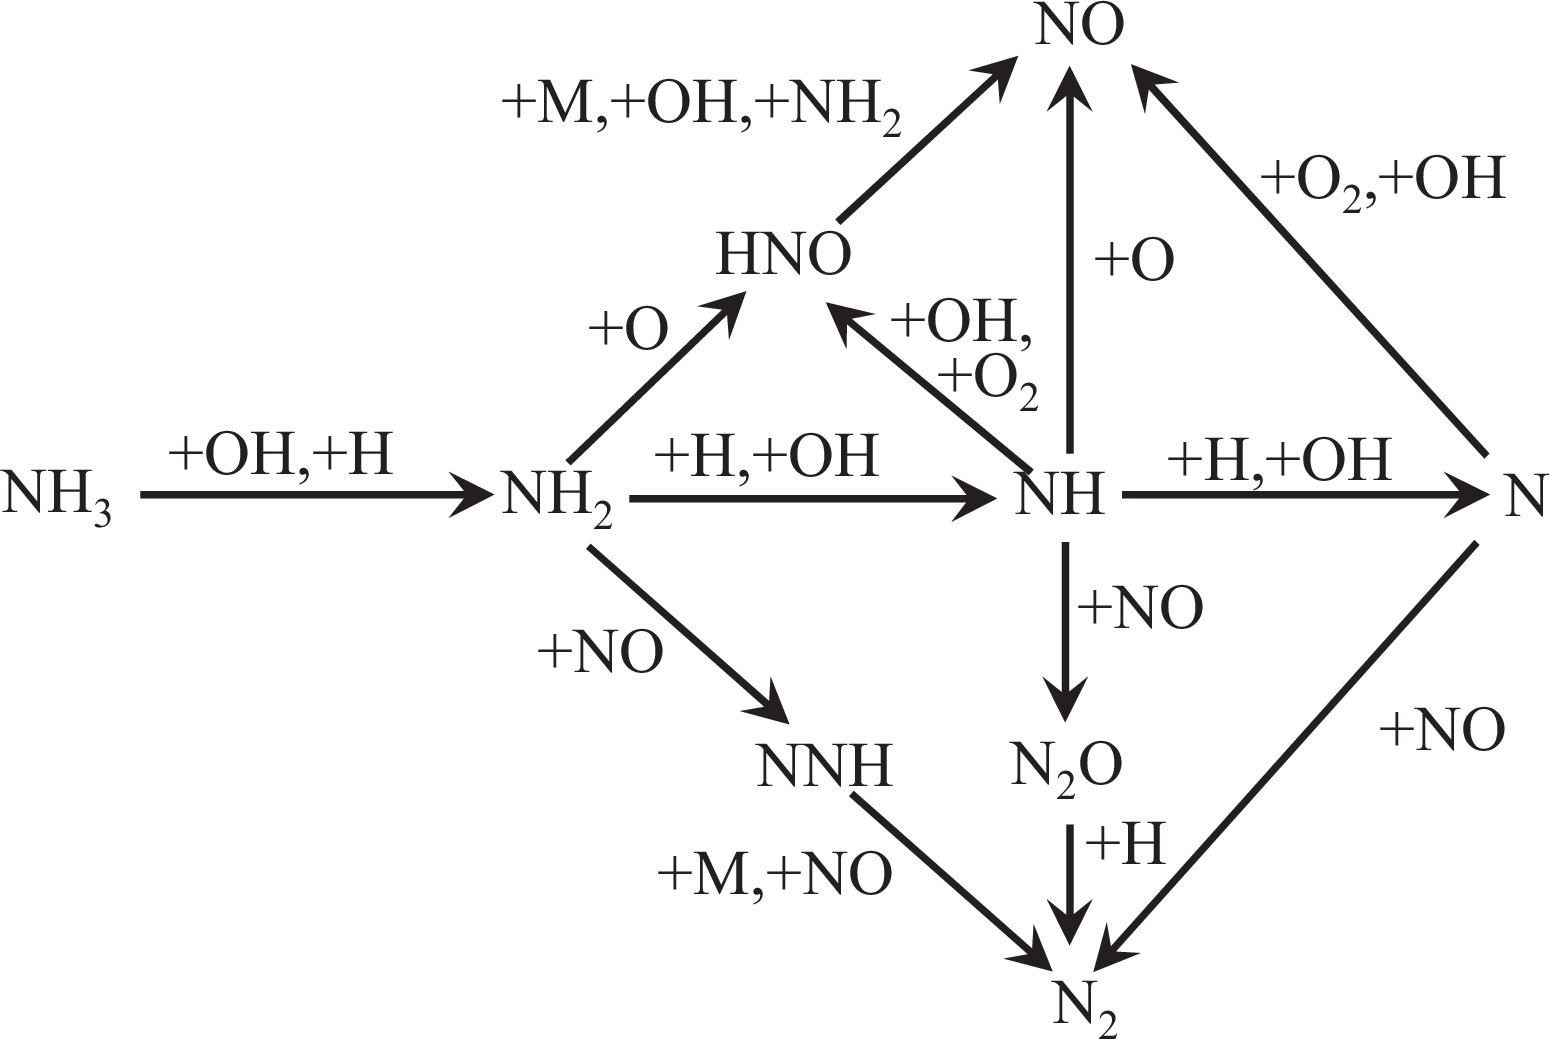
\includegraphics[width=0.6\textwidth]{img/NOx-emission-diagram.jpg}
        \caption{$\mathrm{NH_3}$ oxidation pathway}
    \end{figure}

\end{frame}



\begin{frame}

    More of the different types of NOx emissions

    More of the different types of fuel injectors

    Who uses a suitable replacing combution chamber, what's our target?

\end{frame}

\begin{frame}[allowframebreaks]{References}
    \nocite{*}
    \bibliography{references}
\end{frame}

\begin{frame}[standout]
    Questions?
\end{frame}

\begin{frame}[standout]
    Thank you!
\end{frame}

\end{document}